\chapter{Эксперимент СФЕРА-2}

В этой главе приводится идея, мотивация и краткая история развития метода регистрации отражённого черенковского света, который развивается в эксперименте СФЕРА-2; обозреваются проведённые измерения и полученные на сегодняшний день результаты, обосновывается необходимость и основные направление дальнейшей работы; наконец, приводится качественная модель процесса регистрации ШАЛ на этом эксперименте.

\section{Метод регистрации отражённого черенковского света ШАЛ}

\textbf{TBD}: идея Чудакова, Наварро, Тянь-Шань, см. \cite{chernov2015-overview} (эта же работа на англ. \cite{Sphere2015}). Написать про мотивацию для метода: статьи с теоретическими критериями для определения массового состава ШАЛ, например \cite{Anokhina2007}, \cite{Chernov2017-ICRC}

\section{Предварительные результаты}

\textbf{TBD}: см. \cite{Antonov2013}, 

\section{Качественная модель работы детектора}

Опишем на качественном уровне теоретические и методические представления, которые лежат в основе интерпретации данных СФЕРА-2. Для этого проследим, что происходит от развития каскада в атмосфере и до получения файлов с экспериментальными данными.

\subsection{Развитие ШАЛ в атмосфере}

Сколько-нибудь полный обзор теории ШАЛ, и даже черенковского света ШАЛ в отдельности, лежит за рамками данной работы, поэтому изложим только самые общие представления. Широкий атмосферный ливень -- каскад вторичных частиц, вызванный взаимодействием первичной частицы большой энергии с атмосферой -- развивается в виде тонкого диска заряженных частиц -- адронов, мезонов, лептонов, гамма-квантов. Черенковский свет -- одно из сопутствующих излучений ШАЛ, возникающее при движении заряженных частиц со скоростью, превышающую скорость света в среде распространения. Черенковский свет ШАЛ также распространяется в виде тонкого -- до нескольких метров в толщину -- диска, ориентированного перпендикулярно оси ливня. Для практических задач моделирование процессов развития ШАЛ проводится численно, например, с помощью программы CORSIKA \cite{CORSIKA-report}.

Уже на этапе моделирования ШАЛ закладывается ряд неопределённостей реконструкции параметров первичной частицы. Во-первых, модели ядерного взаимодействия при энергиях $\gtrapprox 10^{16}~\text{эВ}$ не проверены экспериментально, являясь, в сущности, экстраполяциями, и разные такие модели могут приводить к несколько разным картинам развития ливня для одной и той же первичной частицы; во-вторых, развитие ШАЛ -- принципиально стохастический процесс, что приводит к статистической неопределённости любой реконструкции. Эти неопределённости будем в дальнейшем называть \textit{модельными}, так как они напрямую связаны с моделью описываемого явления, в противоположность \textit{инструментальным} неопределённостям, связанным с процессом измерения характеристик ливня.

\subsection{Отражение света от снега}
\label{sect:snow-reflection}

Эксперименты, использующие отражённый черенковский свет, предъявляют особые требования к земной поверхности на уровне наблюдения -- она должна служить <<экраном>>, который бы равномерно и предсказуемо рассеивал свет. В случае СФЕРЫ-2 таким экраном служит заснеженный лёд озера Байкал.

Рассеивающие свойства снега могут существенно повлиять на работу эксперимента, поэтому для измерения и мониторинга этих условий были приложены определённые усилия. В частности, были проведены прямые измерения коэффициента отражения в зависимости от угла \cite[рис.~11]{Sphere2015}, и было обнаружено, что зависимость хорошо согласуется с законом рассеяния Ламберта для идеальной диффузной поверхности: \textit{яркость} рассеянного света не зависит от угла, то есть интенсивность имеет чисто геометрическую зависимость $I \propto \cos \theta_n$ \cite{Antonov2019}. Альбедо $a$ -- отношение падающего и отражённого потоков -- было принято независимым от длины волны \cite{Warren1982} и равным $0.9$.

\subsection{Сбор отражённого света}
\label{sec:light-collection-from-surface}

Установка СФЕРА-2 поднималась аэростатом на высоту $400$ -- $900~\text{м}$, для сбора света с поверхности использовалась оптическая система из диафрагмы, сферического зеркала и мозаики ФЭУ, которая схематично изображена на рис. \ref{pic:sphere-detector-optical-scheme}. В результате каждый из ФЭУ обозревал область на поверхности диаметром $10$ -- $50~\text{м}$.

\begin{figure}
	\centering
	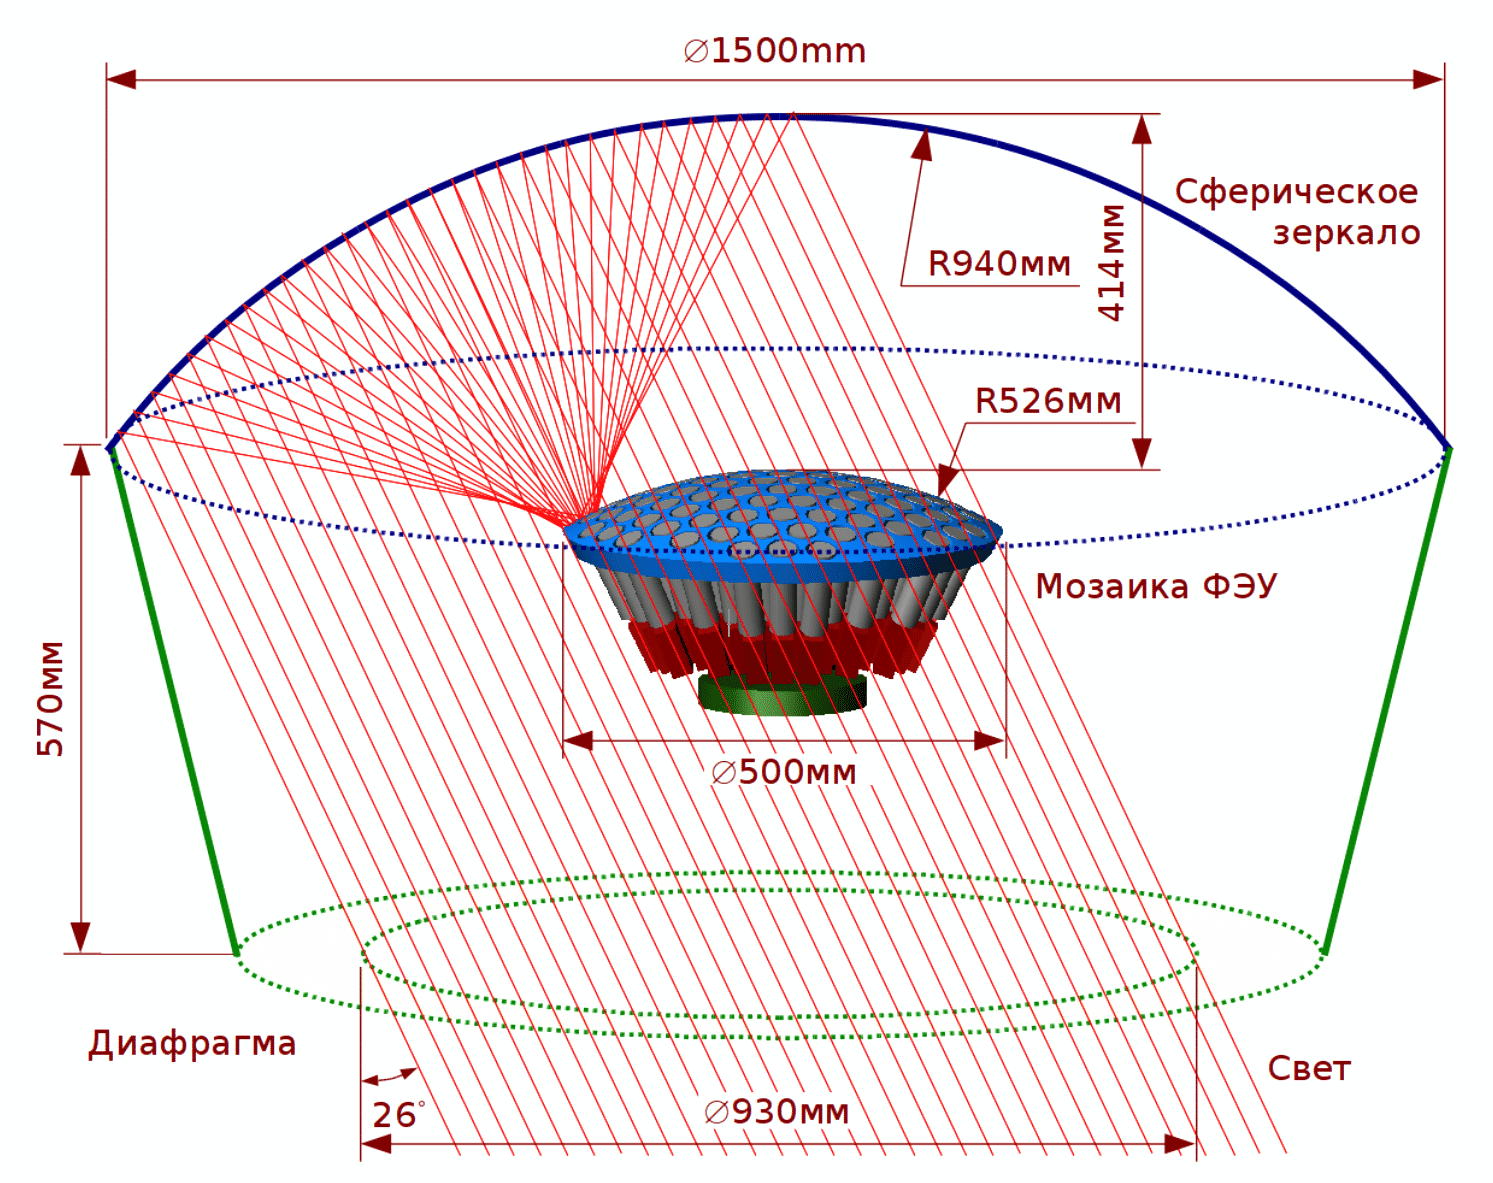
\includegraphics[width=\columnwidth]{optical_scheme}
	\caption{Оптическая схема детектора СФЕРА-2}
	\label{pic:sphere-detector-optical-scheme}
\end{figure}

Качественно оценим коэффициент сбора света: пусть на участок поверхности в окрестности точки $(x, y)$ в системе координат с центром в проекции детектора падает $\delta N_{gr}$ фотонов, и пусть горизонтально ориентированная диафрагма радиусом $R_{d}$, поднята на высоту $H$. Обозначая угол рассеяния света от нормали $\theta_n$, можно оценить число фотонов, которое достигнет диафрагмы из результатов предыдущего раздела и геометрических соображений

\begin{equation}
	\delta N_{d} = \frac{R_d^2 \cos \theta_n}{H^2 + x^2 + y^2} K \cos \theta_n \delta N_{gr}
\end{equation}

Из этого простого расчёта при характерных значениях $H = 600~\text{м}$, $R \approx 0.45~\text{м}$ получается оценка общего коэффициента сбора установки: $(0.5 \div 1) \cdot 10^{-6}$.

Для расчёта количества фотонов, достигающего каждого отдельного ФЭУ, требуется численное моделирование распространения света внутри мозаики, отражения от зеркала, поглощения тыльной стороной мозаики и элементами конструкции. Результатом такого моделирования является коэффициент сбора как функция координат на поверхности, или \textit{чувствительность} каждого ФЭУ $k_i(x, y)$. Более строго, если флюенс черенковских фотонов равен $n(x, y)$, то число ожидаемое число фотонов, попавших в $i$-тый ФЭУ, будет равно $\int_{\infty} k_i(x, y) n(x, y) dx dy$.

Функции $k_i$ имеют форму пятен, соответствующих полям зрения ФЭУ на поверхности льда. Пример нескольких таких пятен, а также суммарной чувствительности всей мозаики для одного из экспериментальных событий изображён на рис. \ref{pic:experimental-pmt-fov-example}. Ясно, что поля зрения зависят от высоты подъёма и ориентации установки, поэтому при расчёте учитывается данные GPS и инклинометра соответственно.

\begin{figure}
	\centering
	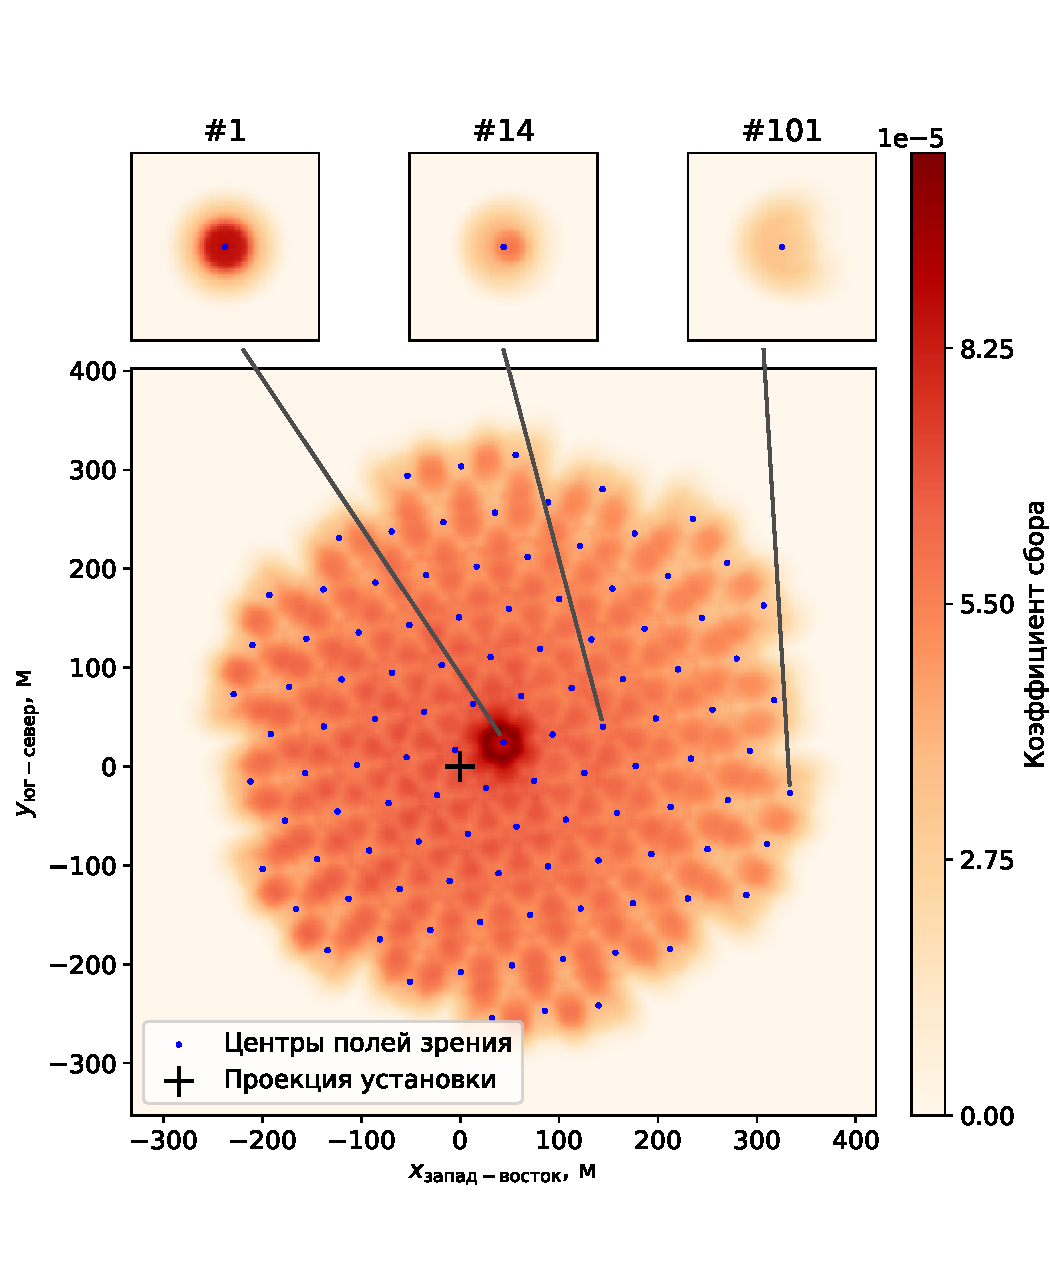
\includegraphics[width=\columnwidth]{experimental-pmt-fov-example}
	\caption{Пример моделирования сбора света с поверхности установкой СФЕРА-2 для экспериментального события \#10699. Показаны чувствительности трёх отдельных ФЭУ и суммарная чувствительность всей мозаики. Учтены данные о высоте подъёма и наклоне установки -- поэтому картина чувствительности сдвинута относительно проекции установки и слегка вытянута.}
	\label{pic:experimental-pmt-fov-example}
\end{figure}

\subsection{Регистрация собранного света}

Финальный этап процесса регистрации события включает несколько подэтапов, которые мы изложим особенно подробно, поскольку именно они обуславливают многие исследуемые в настоящей работе эффекты.

\subsubsection{Мозаика ФЭУ}
\label{sec:pmt-mosaic-details}

Вблизи фокальной поверхности сферического зеркала расположена мозаика из 109 ФЭУ (см. рис. \ref{pic:sphere-detector-optical-scheme}), собранных в приближённо гексагональную сетку. В центре расположен ФЭУ Hamamatsu R3886, характеризующийся б\`{о}льшим коэффициентом усиления, остальные -- ФЭУ 84-3. Hamamatsu использовался как референсный ФЭУ в процессе калибровки детектора \cite{SphereCalibration2016}.

\subsubsection{Рождение фотоэлектронов на фотокатоде ФЭУ}

\label{sec:photon-to-phels-conversion}

Попадая на фотокатод ФЭУ, фотон с определённой вероятностью порождает фотоэлектрон, который затем под действием приложенной разности напряжений устремляется к первому диноду, на котором рождается ещё несколько электронов, и так далее, -- таким образом до анода доходит лавина фотоэлектронов, создающая заряд, достаточный для регистрации. Процесс фотоэффекта характеризуется функцией квантовой эффективности, которая характеризует вероятность, с которой фотон данной длины волны породит фотоэлектрон в системе.

Однако, поскольку отражающая способность снега в принятой модели (см. \ref{sect:snow-reflection}) не зависит от длины волны, спектр черенковских фотонов на фотокатоде оказывается таким же, как и в самом ливне. Поэтому для сокращения объёма данных при моделировании ШАЛ паспортная квантовая эффективность ФЭУ была заложена уже на этапе прослеживания ливня в атмосфере -- вместо спектра черенковского света сохранялась его свёртка с кривой квантовой эффективности, дающая ожидаемое число фотоэлектронов. Таким образом, в настоящей работе \textit{фотоны} ШАЛ всегда подразумеваются уже преобразованными в фотоэлектроны описанным способом, поэтому эти термины во многих случаях оказываются взаимозаменяемы, несмотря на фундаментальные физические различия.

\subsubsection{Лавинное усиление ФЭУ}
\label{sec:pmt-amplification-description}

Процесс развития электронной лавины на системе динодов ФЭУ -- принципиально статистический процесс. Это подтверждается прямыми лабораторными измерениями флуктуаций заряда, собранного на аноде Hamamatsu \cite[рис. 9]{SphereCalibration2016}, а также общими представлениями о механизме усиления: если динодная система насчитывает $N \approx 10$ динодов, а общий коэффициент размножения составляет в среднем $K \approx 10^6$, то средний коэффициент размножения на одном диноде будет составлять $\sqrt[N]{K} \approx 4$. Стохастический характер фотоэффекта приводит к тому, что истинный коэффициент умножения на каждом диноде будет иметь пуассоновское распределение с математическим ожиданием $\sqrt[N]{K}$. Эта простая модель позволяет получить распределение коэффициента усиления для ФЭУ84-3, для которого недоступны лабораторные измерения. Результаты этого моделирования и их следствия подробно обсуждаются в разделе \ref{sec:experimental-rir} (см. рис. \ref{pic:experimental-rir-params}).

Ясно, что статистический характер коэффициента усиления ФЭУ не играет большой роли при измерении больших потоков, так как происходит эффективное усреднение этой величины. Не важен он и при малых потоках, когда ФЭУ работает в режиме счёта фотонов и на осциллограмме наблюдаются отдельные хорошо разрешённые импульсы. Однако характерная интенсивность потока фотонов в эксперименте СФЕРА-2 такова, что режим работы попадет между этими двумя -- поток уже слишком велик, чтобы нельзя было разрешить отдельные фотоны, но ещё недостаточен, чтобы произошло эффективное усреднение. Именно этим обусловлена необходимость статистической деконволюции, описанной в главе \ref{chapt:bayesian-deconvolution}.

\subsubsection{Оцифровка импульса анодного тока}

Учитывая описанные условия, можно качественно охарактеризовать анодный ток ФЭУ. С одной стороны, постоянный поток фоновых фотонов -- преимущественно звёздного и зодиакального света, будут приводить к наличию стационарного тока. С другой стороны, фотоны ШАЛ, приходящие короткой сконцентрированным во времени пакетом, будут давать более и менее яркий импульс на этом фоне. Важный качественный результат лабораторных измерений состоит в том, что другие источники шума -- темновой ток или другие электронные шумы -- пренебрежимо малы по сравнению с сигналом от фоновых фотонов, поэтому в дальнейшем они учитываться не будут.

Подробное описание электроники детектора может быть найдено в работе \cite{SphereDetector2020}, здесь же ограничимся качественной картиной: постоянная и импульсная компоненты анодного тока разделяются RC-фильтром и записываются отдельными АЦП. Частота дискретизации для импульсной компоненты составляет $12.5~\text{нс}$, для постоянной -- показания АЦП сохраняются поминутно.

\subsubsection{Линейность}

Линейность системы регистрации света (связки ФЭУ и считывающей аппаратуры) была отдельно исследована по калибровочным кадрам. Интенсивность света в них намного выше даже самого яркого события ШАЛ, но даже в этих условиях амплитудная характеристика остаётся весьма близка к линейной, и может быть подвергнута дополнительной коррекции \cite[рис. 6]{SphereCalibration2016}. Поэтому в дальнейшем система регистрации света считается линейной.
